\documentclass{article} % For LaTeX2e
\usepackage[utf8x]{inputenc}
\usepackage[T1]{fontenc}
\usepackage{nips11submit_e,times}
\usepackage{natbib}
\usepackage{amsmath}
\usepackage[pdftex]{graphicx}
\usepackage{verbatim}
%\documentstyle[nips10submit_09,times,art10]{article} % For LaTeX 2.09


\title{A Common GPU n-dimensions array}


\author{
Frédéric Bastien, Arnaud Bergeron, Pascal Vincent and Yoshua Bengio \\
D\'epartement d'Informatique et de Recherche Op\'erationnelle\\
Universit\'e de Montr\'eal\\
Montr\'eal, Canada \\
\texttt{\{bastienf, bergearn, vincentp, bengioy\}@iro.umontreal.ca} \\
}

% The \author macro works with any number of authors. There are two commands
% used to separate the names and addresses of multiple authors: \And and \AND.
%
% Using \And between authors leaves it to \LaTeX{} to determine where to break
% the lines. Using \AND forces a linebreak at that point. So, if \LaTeX{}
% puts 3 of 4 authors names on the first line, and the last on the second
% line, try using \AND instead of \And before the third author name.

\newcommand{\fix}{\marginpar{FIX}}
\newcommand{\new}{\marginpar{NEW}}

\nipsfinalcopy % Uncomment for camera-ready version

\begin{document}


\maketitle

\begin{abstract}
Currently there are multiple incompatible array/matrix/n-dimensional object implementations that exist for GPUs. 
This hinders the sharing of GPU code and causes duplicate development work.
This paper proposes and presents a first version of a common GPU n-dimensional array(tensor) named GpuNdArray ~\citep{GpuNdArray} that works with both CUDA and OpenCL. 
It will be usable from python, C and possibly other languages.
\end{abstract}

\section{Introduction}
There are at least 4 different GPU array implementations in
python: CudaNdarray(Theano)~\citep{bergstra+al:2010-scipy},
GPUArray(PyCUDA)~\citep{kloeckner_pycuda_2009},
GPUArray(PyOpenCL)~\citep{kloeckner_pycuda_2009} and
CUDAMatrix(cudamat)~\citep{cudamat-TR2009}. 
There are also other implementations like Trust~\citep{Thrust} in C++. 
One problem is that they are incompatible with each other. 
Each of them implements a different subset of the features that Numpy~\citep{numpy-2007} provides on the CPU, namely a tensor object (arbitrary-dimensional array) with support for \emph{strides}~\footnote{
\emph{Strides} are a way to specify for each dimension in an n-dimensional array a subrange and the number of elements to skip when going
to the next element. 
This allows to operate on a view of the data that represents, say, only odd rows of a matrix without copying any data.
The part to view in each dimension is specified as a range of elements, with a step between each element.
This is represented by a slice with an inclusive start index, an exclusive end index and a step.
}
and \emph{broadcasting}~\footnote{
\emph{Broadcasting} is a generalization of element-wise operations on tensors that extends certain dimensions to fit the required shape.
For example, this allows adding a vector to all columns of a matrix.
Not all existing GPU array implementations support this very useful construct.
It is however easy to add when we have strides support.
}.
Some implementations support only vectors or matrices, some support only \emph{float32}\footnote{
\emph{float32} corresponds to single precision floating point numbers.
}, only contiguous memory layout, etc$\ldots$
None of them targets both CUDA and OpenCL.

The goal is to have a common GPU object that we hope will be used by everybody with the following conditions:

\begin{itemize}
\item Make a n-dimensional array on the gpu that supports strides and broadcasting
\item Don't make development harder with this n-dimensional array. 
\item Make the python interface similar to numpy.ndarray
  \begin{itemize}
  \item Easier to attract other people from python community
  \end{itemize}
\item Have the base object in C to allow collaboration with other non-python projects.
  \begin{itemize}
  \item We want people from C, C++, ruby, R, etc... to all use the same base Gpu ndarray.
  \end{itemize}
\item Be compatible with CUDA and OpenCL
\end{itemize}

We believe that for a common GPU object, an n-dimensional array is required.
The motivation is that forcing users to use an object that supports only a certain number of dimensions adds complexity when dealing with algorithms that need more than what is supported.
We don't think that this complexity should be dealt with by each user and having a base object that supports n-dimensions, eliminates this complexity.
We believe that there are several reasons why there has not yet been a common GPU implementation fulfilling our objectives.

One may be that such a general tensor implementation on GPU is hard and time consuming to get right and efficient.
Since support for general memory layout is time consuming and sometimes impossible, we will provide functions to convert any tensor to a desired memory layout.  This can be used by kernels that support only a certain layouts to convert their inputs.

Another reason may be that support for additional dimensions requires extra computations in the kernel which can more easily overshadow the actual computation on the GPU.
In order to offset this cost, optimizations like the collapsing of dimensions can be done before launching the kernel.  
This is implemented for elemwise operations as discussed in the ``Current implementation'' section.

We think that if we provide such optimized functions for elemwise and reduction operations, we will cover enough cases where the conversion from one memory layout to another can be combined with computations.
This can still impact the performance due to coalescing constraints, but we don't expect that to be significant most of the time.

\section{Existing Implementations}
\subsection{Theano(CudaNdarray)}
Theano is the system that provides the closest approximation of a GPU tensor. 
According to its web site Theano~\citep{bergstra+al:2010-scipy} is: ``a Python library that allows you to define, optimize, and evaluate mathematical expressions involving multi-dimensional arrays efficiently''.

It implements a GPU tensor with strides and broadcasting, but supports only float32 and CUDA.
Also, the strides information are stored differently than numpy.
Theano stores the number of elements to skip to access the next element and numpy stores the number of bytes to skip.

\subsection{PyCUDA/PyOpenCL(GPUArray)}
PyCUDA~\citep{kloeckner_pycuda_2009} and PyOpenCL~\citep{kloeckner_pycuda_2009} are python wrappers around CUDA and OpenCL respectively. 
In addition to wrapping their respective library, they do automatic memory management, add a GPUarray object and some abstraction for compilation. 
They also automatically translate errors to python exceptions.

Their GPU array objects are limited to contiguous memory regions.
They add shape properties to allow using this contiguous memory region as n-dimensional array.
They don't support strides or broadcasting, but they support many data types.

\subsection{CUDAMat}
The CUDAMat~\citep{cudamat-TR2009} website describes itself with: ``The aim of the cudamat project is to make it easy to perform basic matrix calculations on CUDA-enabled GPUs from Python. cudamat provides a Python matrix class that performs calculations on a GPU.''

So we clearly see that it supports only CUDA and matrices. 
If we look deeper we see that it doesn't support strides and supports only float32. 
Broadcasting is supported via a function, but not via the usual numpy syntax.

\subsection{Gnumpy}
Gnumpy~\citep{gnumpy-TR2010} is built on top of cudamat.
It works only with contiguous n-dimensional arrays and does not support strides.
It also adds support for the boolean type by using 1.0 and 0.0 in floating point to represent true and false, respectively. 
It also supports broadcasting via the numpy syntax.

\subsection{Trust}
Trust~\citep{Thrust} is a C++ template library.
It provides a vector object for CUDA.
It supports all data types, but only one dimension.
This means no broadcasting and no strides.

\subsection{Summary}
We see clearly that none of those implementations offer all of what we want for a common GPU tensor.
As the Theano implementation supports strides and that it is easier to add other types than to add strides support, we used much of its code as a starting point for our implementation.
Theano also implemented some optimizations to lower the performance loss of having more dimensions.

\section{Current implementation}

We currently have all the code implemented and working for CUDA.
OpenCL is partially implemented and some adjustments remain to be done.

\subsection{Functionality}

The current code can allocate arrays, transfer data to and from the CPU, create views of that data and run elemwise kernels.
In order to support multiple APIs we have created a list of utility functions that are to be implemented for each API and the rest of the code is shared.

The API independent parts take care of indexing, making views, and provide an interface that is very similar to numpy.
This is the part that supports any (valid) combination of dimensions and strides.
Most importantly, the dimension collapsing optimizations are device-independent and can be reused between APIs.

We are still missing some items before we reach full numpy compatibility, most importantly reductions, setting a part of the array via assignation and reshaping.

\subsection{Elemwise dimensions collapsing}

To lower the indexing computation cost with more dimensions, we can try to \emph{collapse} consecutive dimensions for the purpose of doing elemwise computations.
For example, if we add tensors that are C-contiguous, we can use the same kernel for all number of dimensions (effectively collapsing any number of dimensions to 1) since the result will be the same.
This way,  we avoid most of the index computations.

In general any non-strided dimension can be collapsed leaving only the strided dimensions to compute indexing for in the kernel.
So if we have only the last dimension of a tensor that has strides, then we can collapse all the other dimensions (assuming that the other inputs don't have strides) and only do the indexing computations for one collapsed dimension and the original strided one.

\section{Benchmarks}

In order to measure the overhead of indexing computations relative to existing implementations, we compared some elemwise kernels generated with PyCUDA to some generated using our algorithm (including dimension collapsing and strides data).
The timings shown below do not include any transfer time or allocation of output.
They were made on a GeForce GTX 580.

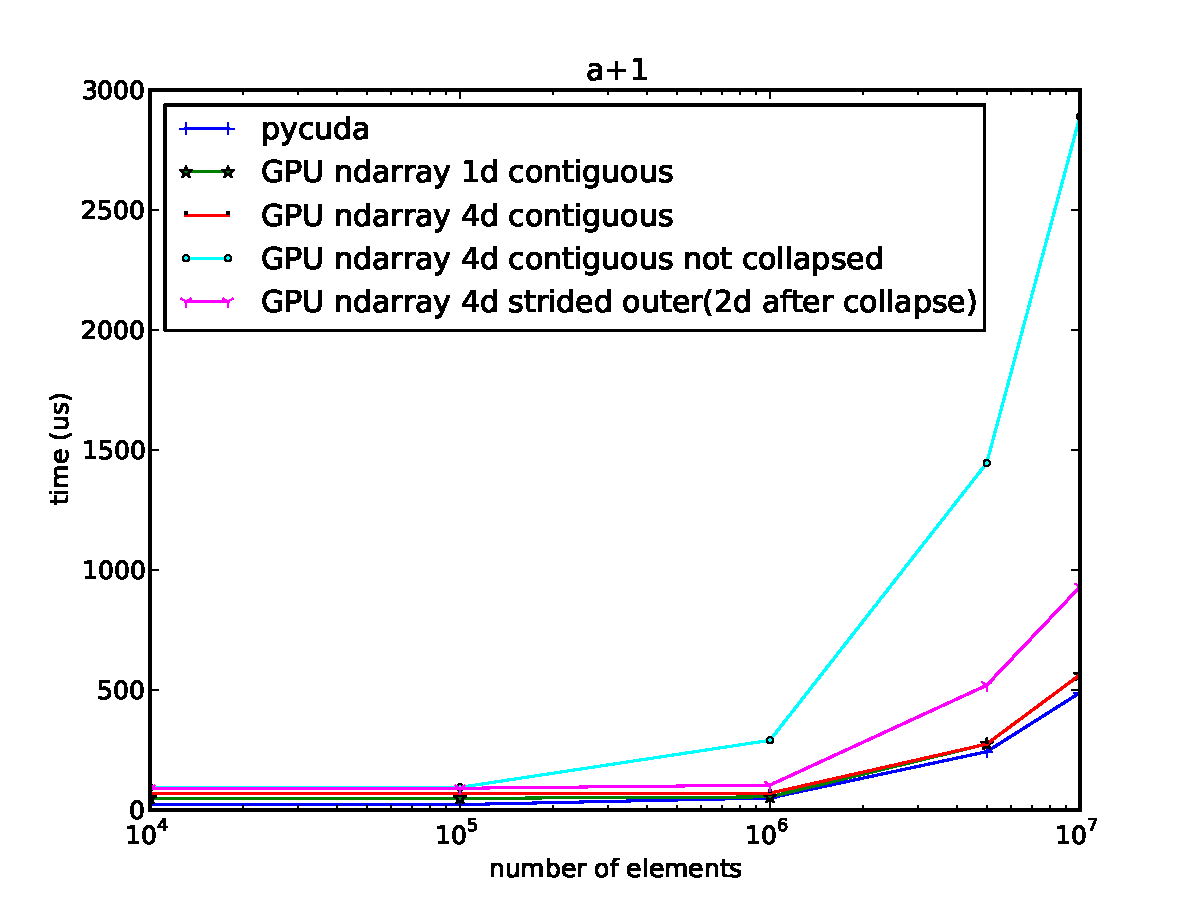
\includegraphics[width=0.495\textwidth]{ap1_no_alloc}
%%\includegraphics[width=0.5\textwidth]{apb_no_alloc}
%%\includegraphics[width=0.5\textwidth]{2ap3b_no_alloc}
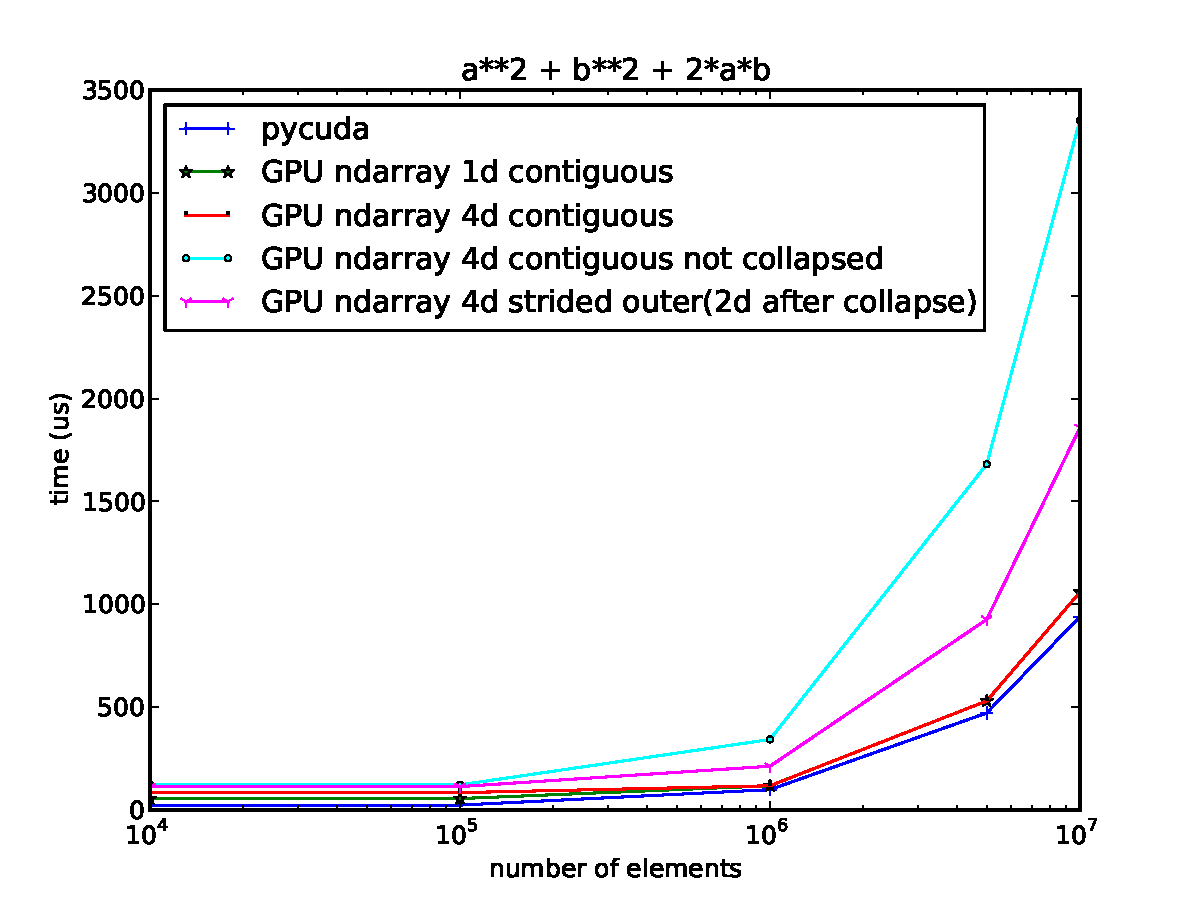
\includegraphics[width=0.495\textwidth]{a2pb2p2ab_no_alloc}

We can conclude from these benchmarks that we have a bigger base cost
that PyCUDA with few elements, but this get not significant with more
elements.  We see clearly that doing the collpsing of dimensions give
a significant speed up by comparing the line "compyte 4d contiguous"
and "compyte 4d contiguous not collapsed". Normally on the gpu,
strided access should lower the speed, but went comparing the line
"compyte 4d strided outer"(collapsed to 2 dimensions) and the line
"compyte 4d coutigious not collapsed" we see that the strided have
less impact that the number of dimensions used in the element wise gpu
function. We currently didn't used implicit loop in CUDA, doing so
would help lower this index computation cost.

TODO: moar stuff

\section{Future Plans}

We plan to continue lowering the overhead as much as possible and to finish the OpenCL side of things.
We also plan to implement reduction operations and to contact people from the C/C++ community to have a good interface available in that language. Make element wise code that use implicit loop in CUDA/PyOpenCL.

Since some Theano authors are working on this project, it will see some usage in a future version. PyCUDA and PyOpenCL, on their side, have already started a branch to use this new object.

\section{Conclusion}

We have explained why we need a gpu n-dimentional array. We have show that we can work around the additional complexity with fonction that will convert memory layout and optimization trick like collapsing of dimensions.

\subsubsection*{Acknowledgments}

We want to thanks James Bergstra. We used some of his code as the first version of some functionality currently implemented. We would also like to acknowledge Compute Canada, RQCHP, NSERC, and Canada Research Chairs for providing fonds or access to compute resources.


\bibliography{strings,strings-shorter,ml,aigaion-shorter}
\bibliographystyle{plain}

\end{document}
